\documentclass[12pt, oneside, a4paper, brazil]{abntex2}
% \usepackage[utf8]{inputenc}
\usepackage[brazil]{babel}
% \usepackage[T1]{fontenc}
\usepackage{fontspec}
\usepackage{setspace}
\usepackage{graphicx}
\usepackage{scalefnt}
\usepackage{float}
\usepackage[a4paper, left=3cm, right=2.5cm, top=3cm, bottom = 2.5cm]{geometry}
\usepackage{hyperref}
\usepackage{listings}
\usepackage{color}
\usepackage{titlesec}
%\usepackage[alf]{abntex2cite}
\usepackage{poker}
% \usepackage{times}
\usepackage[scaled]{helvet}
\usepackage{fancyhdr}

\titulo{Implementação de um jogo de bisca utilizando linguagem C}
\autor{Atílio Antônio Dadalto \par Leandro Furlam Turi}
\local{Vitória}
\data{2019}
\instituicao{Universidade Federal do Espírito Santo \par Departamento de Informática}
\tipotrabalho{Relatório}
\preambulo{Relatório apresentado como requisito parcial para obtenção de nota na disciplina de Estruturas de Dados, pela Universidade Federal do Espírito Santo.}

%--- Ajusta tamanho de títulos ---
\renewcommand{\ABNTEXchapterfontsize}{\normalsize}
\renewcommand{\ABNTEXsectionfontsize}{\normalsize}
\renewcommand{\ABNTEXsubsectionfontsize}{\normalsize}

%--- Configurações do environment lstlisting ---
\newfontfamily{\consolas}{Consolas.ttf}

\definecolor{gray}{rgb}{0.5,0.5,0.5}

\lstset{
  language=C,
  basicstyle=\footnotesize\consolas,
  numbers=left,
  numberstyle=\tiny,
  frame=tb,
  tabsize=4,
  breaklines=true,
  postbreak=\mbox{\textcolor{red}{$\hookrightarrow$}\space},
  columns=fixed,
  showstringspaces=false,
  showtabs=false,
  keepspaces,
  commentstyle=\color{gray},
  keywordstyle=\color{blue}
}

%--- Fim do preâmbulo

\begin{document}

\imprimircapa

\imprimirfolhaderosto


\tableofcontents*

%--- Começo do documento ---

\chapter*{INTRODUÇÃO}
\addcontentsline{toc}{chapter}{INTRODUÇÃO}
\textual

Este trabalho tem por objetivo a implementação de um jogo de biscas capixaba de dois ou quatro jogadores, permitindo ao usuário escolher sua posição na mesa de jogo e, assim, promover uma competição Humano \textit{versus} Computador, em dois modos de jogo, seguindo as regras descritas no Capítulo~\ref{cap:1}.

As referências para os Tipos Abstratos de Dados que serão implementados podem ser encontrados nas notas de aula utilizadas pela disciplina, encontradas na \href{https://ava.ufes.br/course/view.php?id=2447}{página da disciplina no AVA}.

O algoritmo foi construído procurando implementar a abstração encontrada pelos autores, descrita no Capitulo \ref{cap:2}, através do Tipo Abstrato de Dado apresentado em sala de aula que mais se aplicasse à estrutura criada, descrito no Capítulo \ref{cap:3}.

Por fim, apresentamos um resumo das principais implementações produzidas no Capítulo \ref{cap:4}, com as principais funções de complexidade no Capítulo \ref{cap:7}, e exibimos a lógica utilizada para as jogadas do Computador em cada modo de jogo no Capítulo \ref{cap:5}. Após, é explicado como funciona a dinâmica do jogo e a maneira correta de se jogar. Entretanto, é aconselhável que se aprenda a jogar no próprio jogo, onde é trabalhado de maneira explícita os passos que devem ser seguidos.

\chapter{O JOGO DE BISCA}\label{cap:1}

A Bisca\footnote{Retirado de: \url{https://pt.wikipedia.org/wiki/Bisca}} é um jogo de cartas onde é utilizado o baralho espanhol de 40 cartas, cujo principal objetivo é acumular mais pontos que o(s) adversário(s), baseando-se nas cartas que são pescadas e descartadas. O número de participantes pode variar de 2 até 4 jogadores, sendo que deve-se jogar em duplas quando tiver 4 jogadores.

O jogo possui a seguinte dinâmica: após um dos jogadores embaralhar e a pessoa ã sua esquerda cortar, uma carta é retirada do baralho e seu naipe determinará o trunfo. Trunfo é o naipe que vai predominar sobre os outros naipes, quando as cartas descartadas forem recolhidas.

Durante o jogo, a carta-trunfo fica embaixo do baralho, mas de maneira visível. Então, são distribuídas três cartas para cada jogador. O jogador que estiver à direita de quem embaralhou baralho começa descartando uma carta, das três que recebe no início do jogo. Em seguida o adversário descarta uma de suas cartas, que vai determinar se ele pega ou entrega as cartas da mesa, baseando-se nos seguintes critérios:

\begin{itemize}
    \item Se as cartas são do mesmo naipe, a carta de maior valor (ou maior número para cartas sem valor de contagem) vence, e o quem a jogou leva as cartas da mesa;
    
    \item Se as cartas são de naipes diferentes e não há um "trunfo" entre elas, quem jogou a primeira carta leva as cartas da mesa;
    
    \item Se as cartas são de naipes diferentes e há um "trunfo" entre elas, quem jogou o trunfo leva as cartas da mesa;
    
    \item Se as todas as cartas são trunfos, a decisão é como o primeiro critério.

\end{itemize}

Após serem recolhidas as cartas (cada jogador tem 2 cartas na mão, nesse momento), os jogadores pegam uma nova carta no baralho (primeiro o jogador que levou as cartas da mesa) e isso se repete até que se terminem as cartas do baralho. Ao final do jogo, contam-se os pontos somando-se as cartas obtidas. Como a pontuação máxima é 120 pontos, um jogador que acumular 61 ou mais pontos antes do jogo terminar já é o vencedor e ganha 1 ponto na partida. A contagem é baseada no valor das cartas, que é crescente: Q (Dama), J (Valete), K (Rei), 7, A (Ás), que valem, respectivamente, 2, 3, 4, 10 e 11 pontos. As cartas de 2 a 6 valem zero pontos.

A bisca pode ser jogada em duplas, onde cada jogador fica de frente para o seu par. No jogo de duplas, é comum que cada jogador mostre suas cartas ao parceiro na primeira e última rodada.

\chapter{ABSTRAÇÃO DO PROBLEMA}\label{cap:2}

\begin{figure}[H]
    \centering
    \caption{Abstração do funcionamento de uma partida de biscas.}
    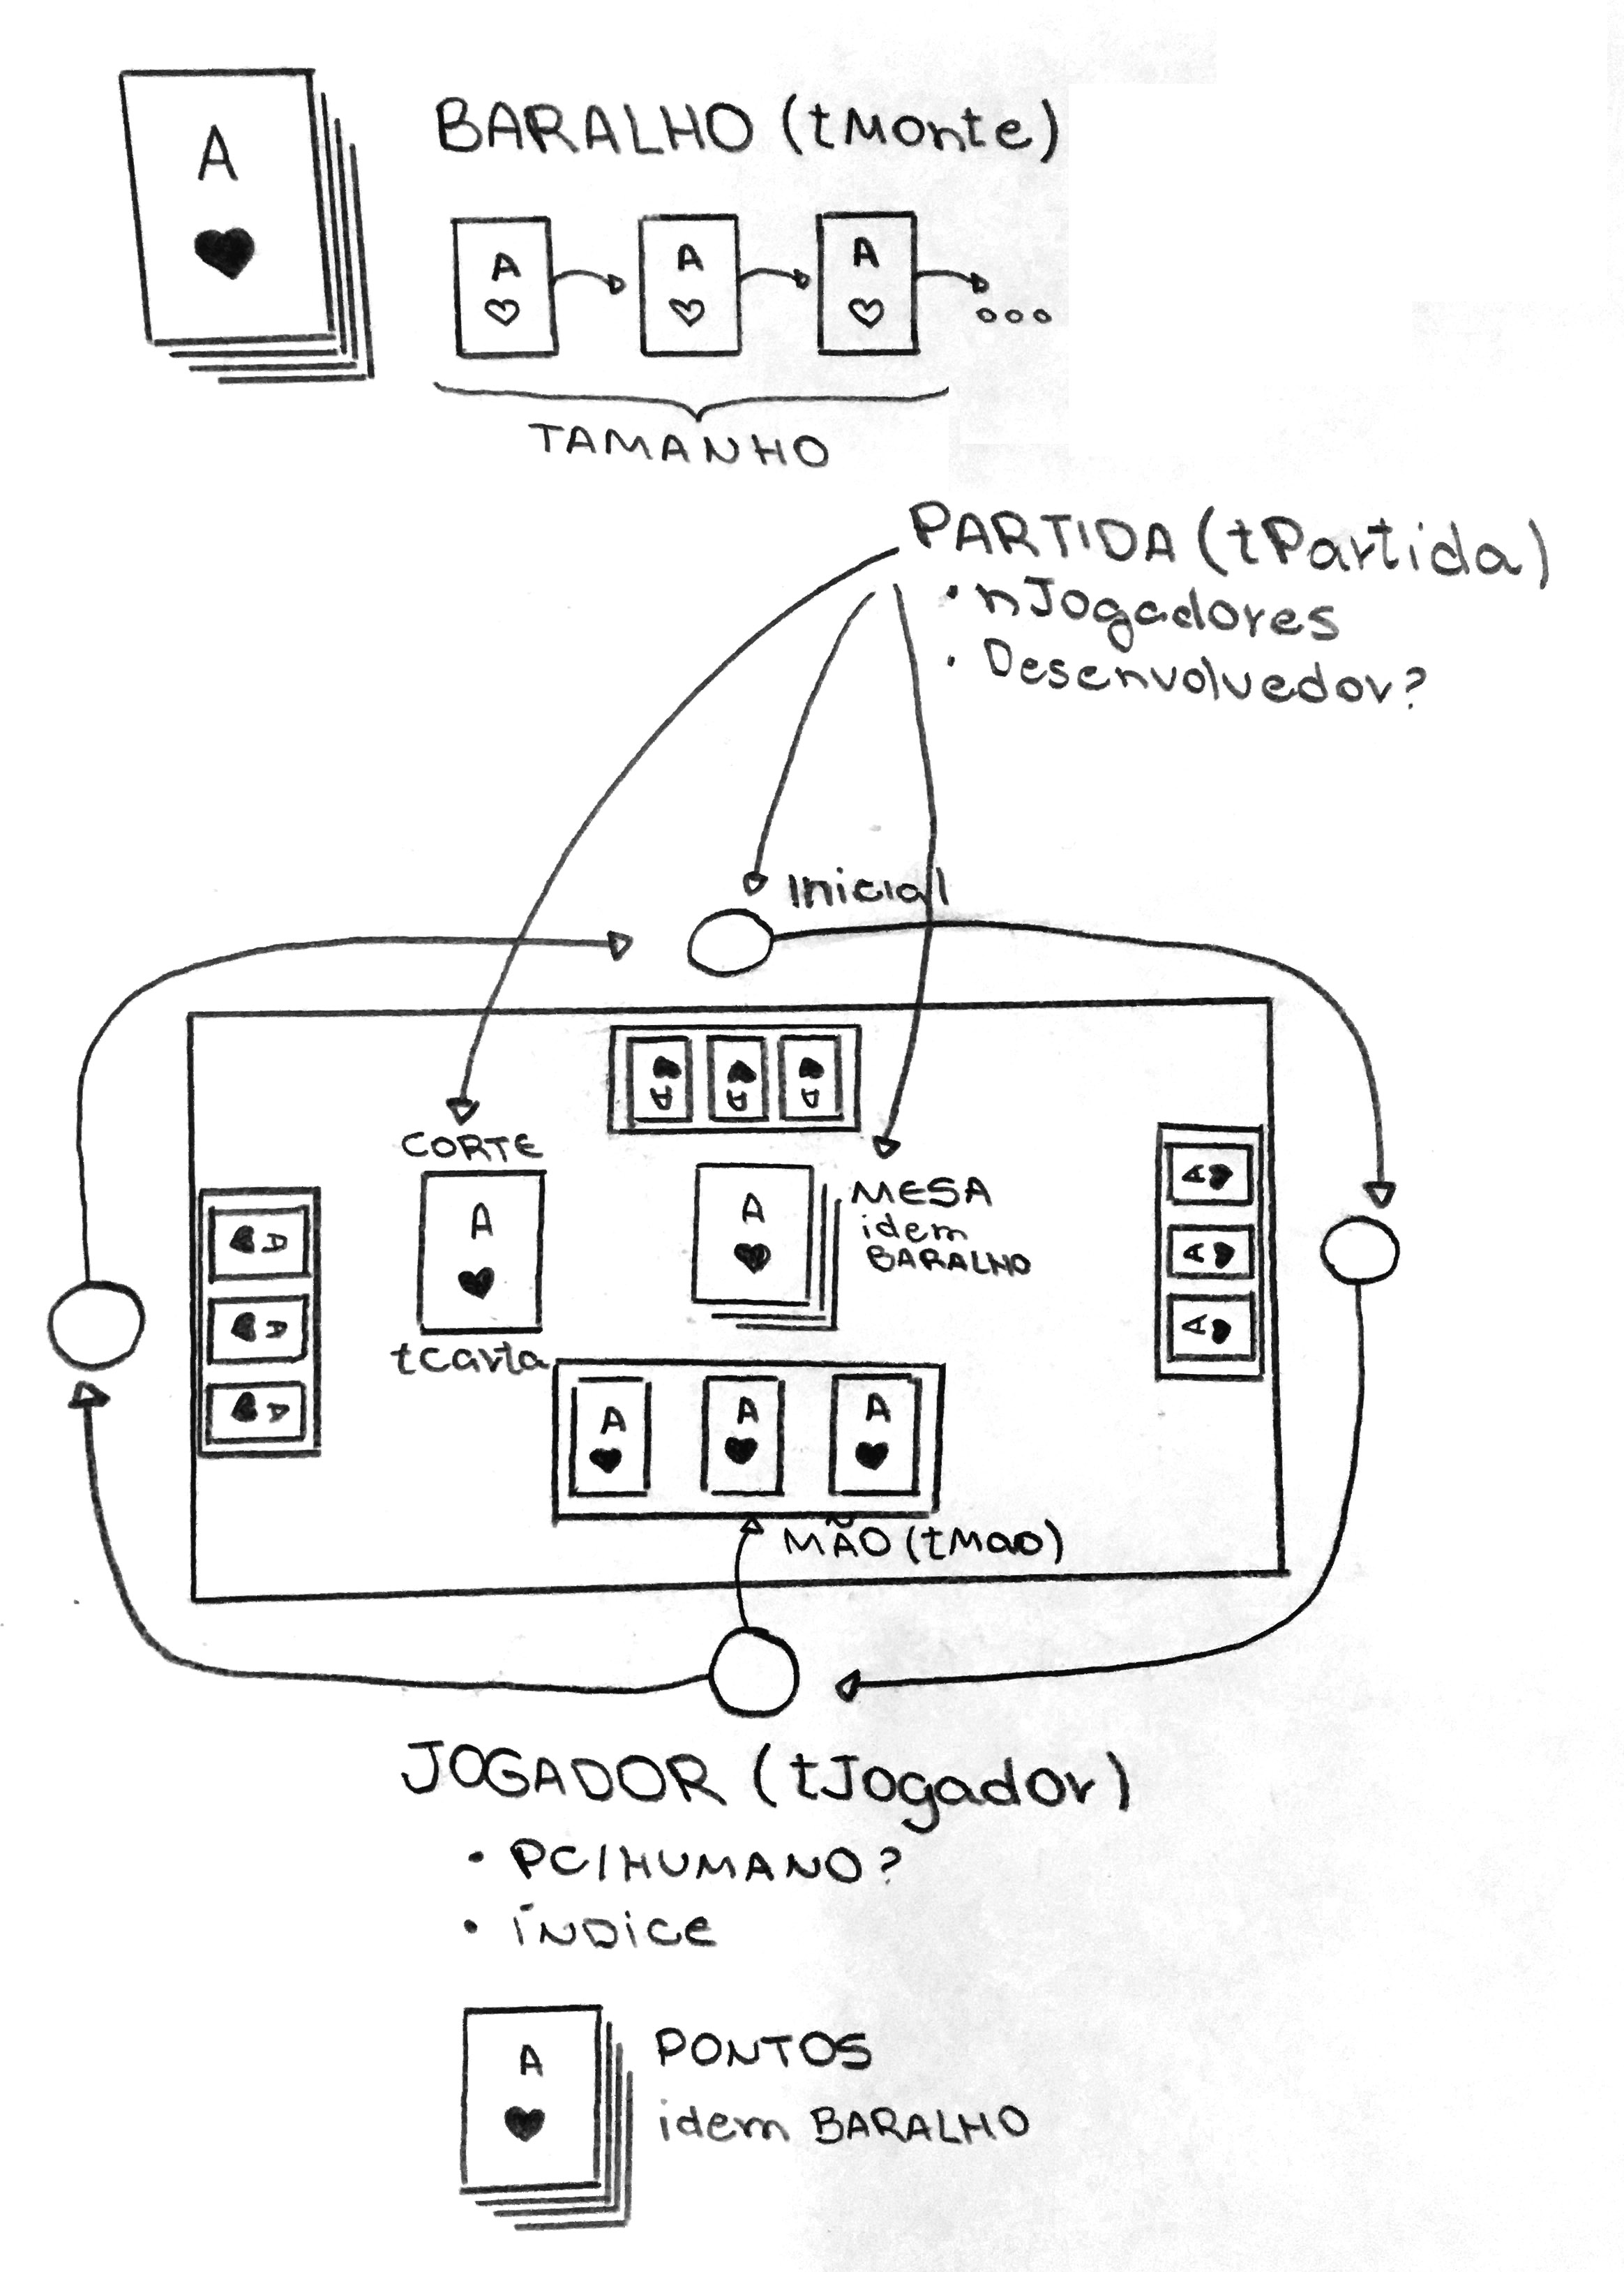
\includegraphics[scale=0.185]{imagens/modo.jpg}\\
    \small{Fonte: elaborado pelos autores.}
    \label{fig:modo}
\end{figure}

No que tange a abstração do problema, representada na Figura \ref{fig:modo}, procuramos decidir, entre os Tipos Abstratos de Dados (TADs), os que melhor se adaptassem ao fragmento do problema proposto. Dessa forma, foi decidido trabalhar com a mão dos jogadores como sendo um TAD listas simples, os montes de cartas que compõe o baralho, as cartas jogadas na mesa e os montes de pontos dos jogadores como TAD listas encadeadas, e os jogadores como um TAD lista circular, onde o jogador inicial seria apontado pela estrutura que compõe a partida.

Como mencionado, para a mão ficou decidido uma implementação de lista simples, pois a ordem das cartas não importa, somente a quantidade de cartas. Os jogadores, a todo momento do jogo, ficam trocando e colocando as cartas em ordens aleatórias, sem se importar com a ordem de chegada das cartas na mão. É muito comum também, aos jogadores mais habituados com a bisca, segurarem as cartas com ambas as mãos, ou unir todas como se fosse uma única carta, ou até mesmo as ordenar com uma sequência de sua preferência. Pela falta de padrão na sequência e ordenamento das cartas na mão, foi decidido essa estrutura.

Quando as cartas possuem uma ordem lógica, foram implementadas com um TAD lista encadeada. No caso do baralho, essa estrutura se mostrou essencial, uma vez que, após embaralhadas, as cartas devem permanecer naquela ordem até o fim do jogo e, mais que isso, cada carta sucede uma carta anterior, formando o monte de cartas. No caso da mesa com as cartas jogadas pelos participantes, foi decidido por essa estrutura pois é necessário saber a ordem que as cartas foram jogadas, para determinar qual é a carta dominante. Por exemplo, caso um jogador, sendo o primeiro, jogue um cinco de espadas, e o trunfo do jogo seja copas, esta carta prevalecerá, a não ser que seja jogado um trunfo ou uma carta de maior valor. Para sabermos sempre qual foi a primeira carta, que é conhecida como caída, a estrutura se tornou necessária. No caso do monte de pontos, foi decidido essa estrutura uma vez que não é conhecida a quantidade de cartas que cada jogador vá pegar, que pode variar de zero a quarenta cartas para cada jogador. Uma implementação que alocasse quarenta posições para cada jogador seria inviável\footnote{Neste caso, respeitamos um consenso da bisca: o montante de pontos só é computado ao final do jogo. Enquanto o jogo não termina, as cartas do monte de pontos não são mexidas.}.

Quanto aos jogadores, abstraímos a ideia de uma mesa, onde cada jogador conhece seu sucessor, que é constante durante todo o jogo. Devido a isso, os implementamos como uma lista circular. Ainda, cada componente do jogo sabe se é um humano ou o computador, ele conhece seu índice, para fins de organização do jogo, possui sua mão contendo as cartas que podem ser jogadas, e possui um monte de descarte contendo seus pontos.

É importante também destacar a abstração da estrutura carta, componente indispensável no jogo. Foi optado por trabalhar ambas as componentes, valor e naipe, como caracteres para que a implementação fosse de fácil entendimento. Essa estrutura possui um ciclo, de forma abstrata, dentro de cada partida: a carta nasce, é colocada dentro do baralho, para então ser embaralhada. A seguir, passa pela mão do jogador, passa pela mesa, e então para o monte de pontos do jogador campeão daquela rodada. Só então, ao final do jogo, após todos os pontos forem computados, elas são destruídas para uma nova partida.

Quanto à partida, é composta pela quantidade de jogadores, se é em modo desenvolvedor ou não, possui uma cópia da carta cortada, possui um apontador para mesa, e possui um apontador para o jogador inicial, que é modificado, quando necessário, ao início de cada rodada.

\chapter{TIPOS ABSTRATOS DE DADOS DEFINIDOS}\label{cap:3}
Em nossa implementação, buscamos utilizar as diversas estruturas vistas no curso, como as listas simples, também conhecido como vetor dinâmico, e as listas dinâmicas, também conhecidas como listas encadeadas. Para as mãos, vistas na seção~\ref{tadMão}, utilizamos um vetor dinamicamente alocado, e para o baralho e montes de cartas, seção~\ref{tadMonte}, utilizamos uma lista encadeada com sentinela. Todas as estruturas opacas contam com suas funções de acesso, garantindo um bom nível de encapsulamento nas estruturas.

\section{BIBLIOTECAS}
O projeto conta com um total de 7 bibliotecas, sendo 3 focadas nas cartas e baralhos, 2 nas IAs e 2 no jogo de bisca propriamente dito.

\subsection{Cartas}
Na BaralhoEncadeado, temos a definição da lista encadeada e o código que implementa funções mais básicas relevantes ao baralho de uma partida de bisca.
A Cartas define e manipula de cartas, e a MaosSimples define a estrutura da mão, bem como as funções para manipulá-la.

\subsection{IAs}
As IAs foram divididas em uma biblioteca para a partida de 2 jogadores --- IA2Jogadores --- e outra biblioteca para a partida de 4 jogadores --- IA4Jogadores. Essa diferença no número de jogadores cria a necessidade de implementar um novo algoritmo para a IA difícil, já que o comportamento do computador deve variar de acordo com o tipo de partida. No caso da IA aleatória, não é necessário estabelecer duas implementações.

\subsection{Jogo de bisca}
Para a construção de uma partida de bisca, foram definidas mais duas bibliotecas --- a PartidaCircular e a Jogo. A primeira define duas estruturas importantes --- a estrutura tJogador e a tPartida e suas funções relevantes ---  enquanto a segunda apenas estabelece funções importantes para a articulação da partida de bisca.

\section{ESTRUTURA CARTA}\label{tadCarta}

Estrutura de dados que abstrai uma carta, que possui valor e naipe:
\begin{lstlisting}
    typedef struct
    {
        char valor;
        char naipe;
    } tCarta;
\end{lstlisting}

Essa é nossa estrutura mais simples, mas é fundamental para o jogo de bisca. Com ela, poderemos representar uma carta no programa e assim fazer as manipulações necessárias para ser possível jogar.

Para preenchermos uma variável tCarta, lançamos mão do uso da diretiva \texttt{\#define}, como a seguir:
\begin{lstlisting}
    // Valores possíveis para números e naipes das cartas da bisca
    #define VALORES "23456QJK7A"
    #define NAIPES "COPE"
    #define nVALORES 10
    #define nNAIPES 4
\end{lstlisting}


Acessar as posições das constantes VALORES e NAIPES como em um vetor, aliado de nVALORES e nNAIPES, nos permitiu construir o baralho de bisca dentro de funções como a CriaBaralho, em que percorremos VALORES e NAIPES para criar todas as cartas possíveis da bisca. Maior detalhamento na seção~\ref{se:implementaçãoCriaBaralho}.

\section{ESTRUTURA MÃO}\label{tadMão}
Estrutura de dados que abstrai uma mão, que possui cartas:
\begin{lstlisting}
    typedef struct
    {
        tCarta *carta;
        int n;
    } tMao;
\end{lstlisting}

Para a abstração da mão de um jogador, foi empregado um vetor de cartas dinamicamente alocado de acordo com o número máximo de cartas na mão definido pela biblioteca Cartas.h. No caso da bisca, esse valor é 3, pois cada jogador possui, ao máximo, 3 cartas na mão. O valor atual de cartas que a mão possui também é armazenado na estrutura tMão.

\section{ESTRUTURA MONTE}\label{tadMonte}


Lista encadeada que abstrai um conjunto de cartas:
\begin{lstlisting}
typedef struct
{
    int tamanho;
    tCelula *cabeca, *ultimo;
} tMonte;
\end{lstlisting}

Para a estrutura de um conjunto de cartas - monte - definimos uma lista encadeada com cabeça e sentinela na biblioteca BaralhoEncadeado.h. A cabeça permanece vazia e os elementos da lista se encontram depois dessa, sendo inseridos sempre após a sentinela. A estrutura também armazena o tamanho da lista, algo extremamente útil e utilizado diversas vezes ao longo do projeto.

\subsection{Estrutura célula}
\begin{lstlisting}
typedef struct tCelula
{
    tCarta carta;
    struct tCelula *prox;
} tCelula;
\end{lstlisting}
Também definida na biblioteca BaralhoEncadeado.h, temos a estrutura tCelula. Como visto anteriormente, cada elemento da lista é uma célula, que por sua vez é uma estrutura que carrega uma carta e aponta para a próxima célula (se esta existir). Naturalmente, a última célula da lista aponta para NULL.

\section{ESTRUTURA JOGADOR}
Estrutura de dados que abstrai um jogador, que possui mão e pontuação:
\begin{lstlisting}
typedef struct tJogador tJogador;
struct tJogador
{
    int PC;
    int indice;
    tMao mao;
    tMonte pontos;
    tJogador *prox;
};
\end{lstlisting}

Para a abstração dos jogadores, também foi implementada uma lista encadeada, porém desta vez circular e sem sentinela.
Ela armazena o tipo de jogador (humano ou máquina), o índice do jogador na lista, a mão do jogador, o monte de pontos (cartas que o jogador obteve ganhando rodadas) e um ponteiro para o próximo jogador da lista.
Essa estrutura nos permitiu ter um controle muito maior sobre os jogadores da partida, pois muitas informações relevantes, como o tipo do jogador, estiveram a fácil acesso.

\section{ESTRUTURA PARTIDA}
Estrutura de dados que abstrai uma partida, que possui mesa, número de jogadores, corte e jogador inicial da rodada:
\begin{lstlisting}
typedef struct
{
    int nJogadores;
    int modoDev;
    int dificuldade;
    tCarta corte;
    tMonte *mesa;
    tJogador *inicial;
} tPartida;
\end{lstlisting}
Essa estrutura engloba todas as outras estruturas definidas anteriormente e é a estrutura principal de nosso programa.
Nela, armazenamos o número de jogadores, se a partida está em modo desenvolvedor ou não, o nível de dificuldade, o corte da partida, a mesa da rodada o jogador inicial da rodada. Com ela, foi possível montar nosso jogo de bisca com um nível muito maior de organização.


\chapter{PRINCIPAIS IMPLEMENTAÇÕES}\label{cap:4}

\section{CRIAR BARALHO}\label{se:implementaçãoCriaBaralho}.
\begin{lstlisting}
Definição:
void CriaBaralho(tMonte *monte)
{
    FMVazio(monte);
    tCarta atual;

    for (int i = 0; i < nVALORES * nNAIPES; i++)
    {
        atual = PreencheCarta(VALORES[i % 10], NAIPES[i / 10]);
        Insere(atual, monte);
    }
}
\end{lstlisting}

Para criarmos um baralho, precisamos primeiramente de uma estrutura adequada para representá-lo. Esta estrutura foi definida na seção~\ref{tadMonte}.

Tendo a estrutura, é necessário que ela esteja devidamente alocada; garantimos isso por meio da função \textbf{FMVazio}, que inicializa uma lista encadeada do tipo monte. Com a lista bem definida, passamos então a preenchê-la com cartas, como antecipado na seção~\ref{tadCarta}. Estabelecemos um loop for que tem o número total de cartas como número de iterações. Na bisca, trata-se de 40, pois temos 4 naipes e 10 valores de cartas. 

Utilizamos uma variável tCarta auxiliar \texttt{atual} no procedimento, aliada da função \textbf{PreencheCarta}, cujo retorno é uma carta com o valor e naipe dados como entrada. O laço funciona da seguinte forma:

Com \texttt{i} de 0 até 9, varrem-se todos os valores do vetor de caracteres \texttt{VALORES}. O valor acessado em \texttt{NAIPES} será o mesmo e só mudará a cada 10 iterações do for. Sendo assim, teremos todos os valores do primeiro naipe (pela nossa definição de \texttt{NAIPES}, o primeiro naipe será copas $\heartsuit$). As próximas iterações seguem da mesma forma para todos os outros naipes, $\spadesuit \clubsuit \diamondsuit$.

\section{EMBARALHAR}\label{se:implementaçãoEmbaralha}
Com o baralho criado, é fundamental que este seja embaralhado para que tenhamos variedade nas partidas. Para isto, duas funções foram implementadas: a função \textbf{TrocaCarta} e a função \textbf{Embaralha}.
Abordaremos, de início, a \textbf{TrocaCarta}, visto que ela é utilizada pela \textbf{Embaralha}.

\subsection{Função TrocaCarta}
A função \textbf{TrocaCarta} foi criada com um objetivo simples: dada uma célula e uma posição \texttt{pos} na lista encadeada, trocar a carta da célula de entrada com a carta da célula na posição \texttt{pos} na lista encadeada. Inicialmente, idealizamos a troca das próprias células de posição, mas, por questões de simplicidade e segurança, optamos por trocar apenas as cartas.

Implementação:

\begin{lstlisting}
void TrocaCarta(tMonte *monte, tCelula *celula, int pos)
{
    int i = 1;

    if (pos <= QuantidadeMonte(monte))
    {
        tCarta primeiraCarta = Carta(celula);
        tCarta segundaCarta;

        tCelula *atual = monte->cabeca->prox;
        while (atual != NULL && i < pos)
        {
            i++;
            atual = atual->prox;
        }
        if (atual == NULL)
        {
            printf("Nao foi possivel chegar na posicao!\n");
        }
        else
        {
            segundaCarta = Carta(atual);
            celula->carta = segundaCarta;
            atual->carta = primeiraCarta;
        }
    }
    else
    {
        printf("A posicao fica fora do monte.\n");
    }
}
\end{lstlisting}

Partindo do contador \texttt{i = 1} (pois começamos no primeiro elemento) e a pré-condição da posição estar na lista, pegamos a carta da célula de entrada e a armazenamos. 
Daí, percorremos a lista até encontrar a célula na posição dada como entrada. Ao encontrá-la, a segunda carta será obtida desta célula. Assim, substituímos a carta da célula de entrada pela carta recém-obtida e substituímos a carta da célula encontrada pela carta da célula de entrada (não foi perdida pois armazenamos essa carta previamente na variável primeiraCarta).

\subsection{Função Embaralha}
Com a função \textbf{TrocaCelula}, podemos definir a função \textbf{Embaralha}:
\begin{lstlisting}
void Embaralha(tMonte *monte)
{
    int posAleatoria = 0, tamMonte = QuantidadeMonte(monte);

    if (tamMonte != 0)
    {
        struct timeval t;
        tCelula *atual = monte->cabeca->prox;

        gettimeofday(&t, NULL);
        srand((unsigned int)t.tv_usec);
        while (atual != NULL)
        {
            posAleatoria = rand() % (tamMonte + 1);
            if (posAleatoria < 1) // Índice começa em 1
            {
                posAleatoria = 1;
            }

            TrocaCarta(monte, atual, posAleatoria);

            atual = atual->prox;
        }
    }
}
\end{lstlisting}
A fim de gerar diferentes números aleatórios a cada execução do software, precisamos inicializar a função \texttt{srand} da biblioteca padrão \texttt{time.h} com uma semente que esteja sempre variando. Para isso, utilizando a estrutura \texttt{timeval} da \texttt{sys/time.h} e a chamada \texttt{gettimeofday(\&t, NULL)}, podemos usar microssegundos como sementes para a \texttt{srand}. Feito isso, mesmo que os números gerados sejam apenas pseudoaleatórios, temos um excelente resultado para o nosso objetivo.

Para embaralhar de fato, partimos da pré-condição de que o monte não está vazio. Então percorremos a lista encadeada gerando posições aleatórias de 1 até o tamanho do monte (inclusive), trocando as cartas das células utilizando a função \textbf{TrocaCarta}. Dessa forma, teremos passado por todas as células e trocado as cartas destas por cartas de células de posições aleatórias. Mesmo que alguma posição aleatória se repita ou que ela já seja a posição da célula \texttt{atual}, conseguiremos embaralhar o monte.

\section{CORTAR} \label{se:cortar}

Após embaralhar, uma quantidade \texttt{pos} de cartas são retiradas e são adicionadas embaixo do monte, seguindo a ordem inicial. Após, é retirada a primeira carta do monte, cujo naipe determinará o trunfo do jogo. Essa carta é adicionada ao fundo do monte, de maneira que fique visível, enquanto as demais não estão visíveis. Trunfo é o naipe que vai predominar sobre os outros naipes, quando as cartas descartadas forem recolhidas. A implementação é definida da seguinte forma:

\begin{lstlisting}
tCarta Corta(tMonte *monte, int pos)
{
    tCarta corte;

    if ((pos >= 1) && (pos <= QuantidadeMonte(monte)))
    {
        int i = 1;
        tCelula *atual;
        atual = monte->cabeca->prox;

        while (atual != NULL && i < pos)
        {
            i++;
            atual = atual->prox;
        }

        if (atual != NULL)
        {
            monte->ultimo->prox = monte->cabeca->prox;
            monte->cabeca->prox = atual->prox;
            monte->ultimo = atual;
            atual->prox = NULL;
            corte = Carta(monte->ultimo);
        }
        if ((Valor(corte) == 'A') || (Valor(corte) == '7')) {
            pos = ((pos + 1) % QuantidadeMonte(monte)) + 1;
            corte = Corta(monte, pos);
        }
        return (corte);
    }
    printf("ERRO! Nao foi possivel cortar.\n");
    return (CartaVazia());
}
\end{lstlisting}

Nota-se que cartas cujos valores são A e 7 não podem ser escolhidas como trunfo. Caso isto ocorra, é escolhida a próxima carta do monte, de maneira invisível aos jogadores da partida, chamando novamente a função de maneira recursiva.

\section{MONTE PARA MÃO}\label{se:implementaçãoMonteParaMao}
As duas próximas funções abordadas fazem a ponte entre listas encadeadas e listas simples, permitindo enviar uma carta de uma lista para a outra.

Implementação da MonteParaMao:
\begin{lstlisting}
void MonteParaMao(tCarta *carta, tMonte *monte, tMao *mao)
{
    tCarta retirada;

    Retira(*carta, monte, &retirada);
    ColocaNaMao(retirada, mao);
}
\end{lstlisting}
A \textbf{MonteParaMao} é a função que envia uma carta de um monte para uma mão. Retira-se a carta do monte e, com a carta retirada armazenada, usamos a função \textbf{ColocaNaMao} para inseri-la na mão desejada. Note que não é necessário usara a variável \texttt{retirada}, pois a carta é dada como entrada, mas deliberamos por essa implementação.

\section{MÃO PARA MONTE}\label{se:implementaçãoMaoParaMonte}
Implementação:
\begin{lstlisting}
void MaoParaMonte(tCarta *carta, tMonte *monte, tMao *mao)
{
    RetiraDaMao(*carta, mao);
    Insere(*carta, monte);
}
\end{lstlisting}

A função \textbf{MaoParaMonte} é análoga à \textbf{MonteParaMao}; é a função que envia uma carta de uma mão para uma monte. Retira-se a carta da mão para então usarmos a função \textbf{ColocaNaMao} a fim de inserir a mesma carta no monte desejado.

\section{ORDENA MÃO} \label{se:ordenamao}

Para ordenar a mão dos jogadores de forma que a implementação das jogadas do computador fossem construídas de maneira mais simplificada, foi implementado o algoritmo de ordenação \textit{bubble sort}, onde, uma vez que os valores, representados por caracteres, não apresentam ordem crescente ou decrescente, é dado um índice a cada valor, conforme são escolhidos os termos do algoritmos da ordenação. Como a mão é de tamanho pequeno, não houve tantas perdas com essa implementação.
O algoritmo ordena os valores de ordem crescente, e em caso de cartas com mesmos valores, é mantido os naipes em sua ordem original.

\begin{lstlisting}
void OrdenaMao(tMao *mao)
{
    int valori = 0, valorj = 0;
    tCarta aux;

    for (int i = 0; i < (TamanhoMao(*mao)); i++)
    {
        for (int j = 0; j < (TamanhoMao(*mao) - 1); j++)
        {
            for (int k = 0; k < nVALORES; k++)
            {
                if (mao->carta[i].valor == VALORES[k])
                {
                    valori = k;
                }
                if (mao->carta[j].valor == VALORES[k])
                {
                    valorj = k;
                }
            }
            if (valori < valorj)
            {
                aux = mao->carta[j];
                mao->carta[j] = mao->carta[i];
                mao->carta[i] = aux;
            }
        }
    }
}
\end{lstlisting}


\section{PARTIDA} \label{se:partida}

O jogo foi implementado, de uma forma geral, dentro da função \textbf{Partida}. Devido ao seu tamanho e a quantidade de operações condicionais, optamos por apresentá-la de maneira simplificada.

Dentro da estrutura circular de jogadores, o jogador cujo ponteiro de inicial da partida estiver apontando começará jogando. Após, a partida é iniciada e são produzidas novas partidas enquanto não é atingida a quantidade máxima de rodadas. Então o foco da função passa a ser a mesa, onde são perguntados aos jogadores qual carta é escolhida enquanto todos não estiverem jogado. Daí, quem irá jogar é selecionado conforme seu índice que diferencia o humano do computador. Então, é selecionada a carta conforme a posição do jogador dentro da mesa, a quantidade de jogadores e o modo de jogo. Após ser obtida a carta escolhida, o próximo jogador passa a próximo apontado pela estrutura do jogador.
A implementação simplificada é descrita a seguir:

\begin{lstlisting}
void Partida(tPartida *partida, tMonte *baralho)
{
    tJogador *atual;
    
    while (rodadas < (40 / QuantidadeJogadores(partida)))
    {
        jogadas = 0;
        atual = JogadorInicial(partida);
        vez = PC(atual);
        while (jogadas < QuantidadeJogadores(partida))
        {
            switch (vez)
            {
            case HUMANO:
                else
                {
                    escolhida = JogaCartaHumano(partida, atual);
                }
                jogadas++;
                vez = PC(atual->prox);
                break;

            case IA:
                if (Dificuldade(partida) == FACIL)
                {
                    escolhida = PCXJogadoresAleatorio(Mao(atual), Mesa(partida), corte, &seteSaiu);
                }
                jogadas++;
                vez = PC(atual->prox);
                break;
            }
        }
     }
\end{lstlisting}


\section{VENCEDOR}

Para declarar o vencedor da partida, são varridas todas as cartas da mesa, sendo comparadas com a maior carta da mesa, isto é, a carta que irá prevalecer sobre as demais dentro da mesa. Quando a maior carta for igual a carta jogada na posição $i - 1$, o jogador inicial passa a ser esse específico. Isto é feito através da função \textbf{MoveCabeca}, onde é movida a cabeça da partida, isto é, o apontador do jogador inicial, \textit{i} posições.

\begin{lstlisting}
tJogador *Vencedor(tPartida *partida)
{
    for (int i = 0; i < QuantidadeJogadores(partida); i++)
    {
        if (CartasIguais(MaiorMesa(Mesa(partida), Corte(partida)), CartaNoIndice((i + 1), Mesa(partida))))
        {
            MoveCabeca(partida, i);
        }
    }

    return JogadorInicial(partida);
}
\end{lstlisting}


\chapter{PROGRAMA DE JOGO: HUMANO \textit{versus} COMPUTADOR}\label{cap:5}

A implementação das jogadas do computador, componente necessária para o trabalho, foi feita em dois modos: um fácil e outro difícil.

No modo fácil, a carta é escolhida aleatoriamente, somente sendo respeitada a regra de que o ás de trunfo não seja jogado antes do sete de trunfo. Optamos por um modo de jogo simplista, tanto na lógica, quanto na implementação.

Já no modo difícil, foi implementado o modo de jogo dos autores, com seus costumes adquiridos por anos jogando bisca. Em dois jogadores, caso o computador seja o primeiro a jogar, é buscado obter pequenos pontos aos poucos, e caso não tenha, é jogado cartas sem valor. Caso ele seja o segundo a jogar, é buscado maximizar a quantidade de pontos, dando prioridade ao \textit{heley}, quando se joga um ás sobre um sete, ambos de trunfo, ou então com um encarte, quando se joga uma carta de pontos mais alta sobre outra de pontos, acumulando grandes quantidades. É visível na implementação a quantidade de estruturas de laço e condicionais. Elas se tornaram indispensáveis nessa implementação pois a busca sempre é específica: ora buscando a maior carta, ora a menor, ora a que se adapta ao caso proposto. Devido à essa especificidade tamanha, foi optado pelo grande uso dessas estruturas, que em piores casos varrem toda a mão, que possui um tamanho pequeno.

No caso de quatro jogadores, a implementação é análoga, salvo ao caso de que os jogadores de mesma paridade estão em duplas. A partir daí, é buscado tomar os pontos do adversário, com um encarte ou trunfo, ou aumentar a quantidade de pontos de seu parceiro, favorecendo sua dupla. É interessante destacar que caso o computador nesse modo de jogo seja o último a jogar em uma partida de quatro jogadores, não é permitido a ele jogar o sete de trunfo. Essa jogada é conhecida como sete de fundo, e é proibida na maioria das partidas capixabas.

\chapter{JOGABILIDADE}\label{cap:6}
Tendo os TADs definidos no Capítulo~\ref{cap:4}, as IAs do Capítulo~\ref{cap:5}, dentre outras funções implementadas, finalmente torna-se possível jogar uma partida de bisca capixaba.

O software é compatível com Windows e distribuições Linux, tendo sido desenvolvido com as duas plataformas em mente. A diretiva \texttt{\#ifdef} foi de grande valor para tornar o jogo compatível com ambos os sistemas, de forma a não prejudicar nenhum sistema por eventuais entraves postos por incompatibilidades. Não foram realizados testes em sistemas MacOS.

As instruções para executar o aplicativo encontram-se no README.txt, mas vale ressaltá-los neste capítulo. Para jogar, extraia o .zip do repositório em algum diretório do computador e acesse a pasta trab1-ed1 pelo terminal de seu sistema operacional. Estando dentro da pasta, mande o comando \texttt{make play} pelo terminal e o jogo será compilado e iniciará imediatamente.\footnotemark

\footnotetext{A ferramenta Make é parte da GNU Toolchain, normalmente presente em distribuições Linux. No caso de sistemas Windows, é necessário instalar as ferramentas GNU através de pacotes como o MinGW e adicionar o seu caminho na variável de ambiente PATH.}

Todas as entradas do usuário passam por uma validação, de forma que o programa não entre em um loop indesejado ou produza um resultado errôneo caso o jogador entre com um valor inválido, por exemplo se o programa pedir um número de 1 a 4 e o jogador informar uma vírgula ou algum caractere especial.

\section{MODO PADRÃO}
Ao planejar o programa, tínhamos em mente criar dois modos dois modos principais -- o padrão e o desenvolvedor. O desenvolvedor será detalhado na seção~\ref{se:modoDev}; o padrão, voltado para o jogador de bisca, é mais limitado, de forma a realmente simular um jogo de bisca.

Iniciando o jogo, o jogador possui a opção de jogar contra um oponente ou jogar em 4 jogadores. Também é possível escolher a dificuldade das IAs, descritas no Capítulo~\ref{cap:5}, de forma a jogar contra oponentes que jogam cartas aleatórias da mão -- modo intermediário/fácil -- ou que tentam maximizar os pontos em todas as jogadas -- modo difícil. 

Após escolher a dificuldade, o programa irá solicitar ao usuário que escolha qual jogador ele deseja ser (1 ou 2 para 2 jogadores ou 1 a 4 para 4 jogadores). Feito isso, o jogo sorteará qual será o primeiro jogador e o monte de cartas será embaralhado. O jogador à esquerda do que começa jogando fará o corte. Caso não seja o humano, uma carta aleatória será cortada; do contrário, o humano poderá escolher a posição da carta a ser cortada. Em seguida, as cartas serão distribuídas para todos os jogadores e o jogo começará de fato.

Neste modo, durante a partida, o jogador possui apenas duas opções -- pedir instruções sobre a bisca e o programa e jogar uma carta da mão. Até o final da partida, essas serão suas ações disponíveis. No entanto, também são exibidos o número de rodadas restantes, cartas restantes no baralho, quantidade de cartas na mão do jogador, além da situação da mesa (corte e cartas na mesa). As posições ou índices exigidos ao jogador sempre vão de 1 até $n$, não se tratando de índices de vetor, que começam de 0 e terminam em $n - 1$, para um vetor de $n$ elementos. 

Ao final da partida, a pontuação de todos os jogadores é exibida, bem como o(s) vencedor(es) e se o humano ganhou. Após isso, o jogo volta para o menu inicial, e o jogador terá novamente a opção de sair do jogo.

\section{MODO DESENVOLVEDOR}\label{se:modoDev}

Para fins de depuração e testes mais refinados, o modo desenvolvedor foi criado. Nele, o jogador possui uma vasta quantidade de opções durante a partida além das usuais do modo padrão, sendo elas:
\begin{itemize}
    \item Mostrar todas as cartas do monte
    \item Mostrar as cartas de todos os jogadores
    \item Mostrar a pontuação de todos os jogadores
    \item Embaralhar o monte
    \item Cortar o baralho
\end{itemize}
O usuário poderá realizar essas ações quantas vezes desejar. Os demais elementos da jogabilidade permanecem inalterados. 

\chapter{PRINCIPAIS FUNÇÕES DE CUSTO}\label{cap:7}
Neste capítulo, abordaremos o custo computacional de funções definidas e explicadas no Capítulo~\ref{cap:4}. Evidentemente, também será necessário discorrer sobre o custo das funções que essas funções utilizam. Caso o custo de uma função já tenha sido explicado, utilizaremos o resultado diretamente.

\section{CRIAR BARALHO}
\subsection{Função FMVazio}
\begin{lstlisting}
void FMVazio(tMonte *monte)
{
    monte->cabeca = (tCelula *)malloc(sizeof(tCelula));
    monte->ultimo = monte->cabeca;
    monte->ultimo->prox = NULL;
    monte->tamanho = 0;
}
\end{lstlisting}
Pode-se notar facilmente que o número de operações independe da entrada, portanto o custo é $O(1)$.

\subsection{Função PreencheCarta}
\begin{lstlisting}
tCarta PreencheCarta(char valor, char naipe)
{
    tCarta carta;

    carta.valor = valor;
    carta.naipe = naipe;

    return carta;
}
\end{lstlisting}
Mais uma vez, a complexidade será $O(1)$. A função sempre realiza apenas duas operações de atribuição de valor, quaisquer que sejam as entradas.

\subsection{Função Insere}\label{subse:custoInsere}
\begin{lstlisting}
void Insere(tCarta x, tMonte *monte)
{
    if (!ExisteCarta(x, monte))
    {
        monte->ultimo->prox = (tCelula *)malloc(sizeof(tCelula));
        monte->ultimo = monte->ultimo->prox;
        monte->ultimo->carta = x;
        monte->ultimo->prox = NULL;

        monte->tamanho++;
    }
    else
    {
        printf("A carta ja existe no monte.\n");
    }
}
\end{lstlisting}
A função \textbf{Insere} parte da pré-condição de que a carta de entrada não existe no monte. Tirando a pré-condição, temos uma função de complexidade de $f(n) = 1$, visto que o algoritmo sempre adiciona elementos após a sentinela da lista encadeada. Como veremos, essa chamada da \textbf{ExisteCarta} tornará o custo da \textbf{Insere} $O(n)$.

A função \textbf{ExisteCarta} está definida da seguinte forma:
\begin{lstlisting}
int ExisteCarta(tCarta x, tMonte *monte)
{
    if (EstaVazio(monte))
    {
        return 0;
    }
    tCelula *atual = monte->cabeca->prox;

    while (atual != NULL)
    {
        if ((Valor(Carta(atual)) == Valor(x)) && (Naipe(Carta(atual)) == Naipe(x)))
        {
            return 1;
        }
        atual = atual->prox;
    }
    return 0;
}
\end{lstlisting}
A função de pré-condição \textbf{EstaVazio} simplesmente retorna se o tamanho do monte é igual a 0, portanto possui função de complexidade de $f(n) = 1$. Após essa verificação, temos um laço \textit{while}, que poderá percorrer até $n$ elementos de uma lista de tamanho $n$ (excluindo a cabeça). Assim, teremos complexidade $O(n)$.

\subsection{Função CriaBaralho}
Tendo estabelecido os custos acima, poderemos então determinar o custo de complexidade da função \textbf{CriaBaralho}.
Temos um laço \textit{for} com $v * p$ iterações, em que $v$ é o número de valores e $p$ é o número de naipes do jogo em questão. Entretanto, o número de naipes e valores é sempre constante. Disto, temos uma complexidade $O(1)$.

\section{EMBARALHAR}
Uma das principais e mais pesadas funções do projeto, a \textbf{Embaralha} percorre todos os elementos do monte, chamando a função \textbf{TrocaCarta} para cada um deles.

\subsection{Função TrocaCarta}
Definida na seção~\ref{se:implementaçãoEmbaralha}, temos que a função \textbf{TrocaCarta} poderá percorrer a lista inteiramente, pois ela fará a busca pela célula na posição \texttt{pos} de entrada. As demais operações são constantes e independem das entradas. Assim sendo, sua complexidade será $O(n)$.

\subsection{Embaralha}
Visto que a Embaralha percorrerá cada elemento do baralho, trocando este com outro elemento através da função \textbf{TrocaCarta}, temos que o custo de complexidade será composto pelas duas funções, a saber, $O(n * n) = O(n^2)$. As demais operações dentro da \textbf{Embaralha} são constantes e independem das entradas.

\section{CORTAR}

A função \textbf{Cortar} apresentada na seção \ref{se:cortar} é implementada de forma que, dada a posição informada pelo usuário, ela irá percorrer todo o monte de cartas, até chegar na posição definida. Daí, temos que sua complexidade será $O(n)$.

\section{MONTE PARA MÃO}
\subsection{Função Retira}
Implementação:
\begin{lstlisting}
void Retira(tCarta x, tMonte *monte, tCarta *cartaRetirada)
{
    tCelula *atual, *anterior;

    anterior = monte->cabeca;
    for (atual = monte->cabeca->prox; atual != NULL; atual = atual->prox)
    {
        if ((Valor(Carta(atual)) == Valor(x)) && (Naipe(Carta(atual)) == Naipe(x)))
        {
            *cartaRetirada = Carta(atual);
            anterior->prox = atual->prox;
            free(atual);
            monte->tamanho--;
            return;
        }
        anterior = atual;
    }
    *cartaRetirada = CartaVazia();
}
\end{lstlisting}

O laço \textit{for} poderá percorrer a lista toda, partindo do primeiro elemento da lista. Portanto, a tempo de execução dependerá do tamanho do monte de entrada, tornando a função $O(n)$. A função \textbf{CartaVazia} sempre retorna uma carta vazia e é $O(1)$, não alterando a complexidade da \textbf{Retira}.

\subsection{Função ColocaNaMao}
\begin{lstlisting}
void ColocaNaMao(tCarta carta, tMao *mao)
{
    if ((TamanhoMao(*mao) >= nMAO) || (!(CartaValida(carta))) || (EstaNaMao(Valor(carta), Naipe(carta), *mao)))
    {
        return;
    }

    mao->carta[mao->n].valor = carta.valor;
    mao->carta[mao->n].naipe = carta.naipe;
    mao->n++;
}
\end{lstlisting}
A inserção de uma carta na mão realiza acesso direto, sendo $O(1)$, porém as validações anteriores a isso também precisam ser avaliadas. A \textbf{TamanhoMao} simplesmente retorna o campo \texttt{n} da estrutura \texttt{tMao} e é $O(1)$. A \textbf{EstaNaMao} percorre a mão verificando se a carta de entrada existe nessa, logo possui complexidade $O(n)$, pois depende do tamanho da mão de entrada. Por fim, a \textbf{CartaValida} realiza até nVALORES + nNAIPES operações, tendo sua função de complexidade $f(v, p) = (v + p)$. Como são valores constantes, temos que sua complexidade é $O(1)$.

Dessa forma, a complexidade da função \textbf{ColocaNaMao} é $O(n)$.

\section{MÃO PARA MONTE}
\subsection{Função RetiraDaMao}
Implementação:
\begin{lstlisting}
void RetiraDaMao(tCarta carta, tMao *mao)
{
    if (!(EstaNaMao(Valor(carta), Naipe(carta), *mao)))
    {
        return;
    }

    for (int i = 0; i < (TamanhoMao(*mao)); i++)
    {
        if ((Valor(carta) == Valor(PegaCarta(i + 1, *mao))) &&
            (Naipe(carta) == Naipe(PegaCarta(i + 1, *mao))))
        {
            mao->n--;
            for (int j = i; j < (TamanhoMao(*mao)); j++)
            {
                mao->carta[j] = mao->carta[j + 1];
            }
        }
    }
}
\end{lstlisting}    

A função de pré-condição \textbf{EstaNaMao} percorre a mão verificando se a carta de entrada existe nessa, possuindo complexidade $O(n)$, pois depende do tamanho da mão de entrada.
Após isso, teremos um laço \textit{for} de 3 (tamanho da mão) iterações. Para cada iteração, teremos 3 iterações, com \texttt{j} partindo de \texttt{i} até o tamanho da mão. Esse laço é necessário para mover os elementos do vetor após um elemento ter sido retirado.
A \textbf{RetiraDaMao} terá, portanto, função de complexidade $f (n) = (n + 3 * 3)$. Daí, sua complexidade será $O(n)$.

\subsection{Função MaoParaMonte}
O custo da função \textbf{Insere} foi visto na subseção~\ref{subse:custoInsere} e é $O(n)$. Com isso e o custo da \textbf{RetiraDaMao}, concluímos que a função de complexidade da função \textbf{MaoParaMonte} é $ f(n) = (1 + n + v + p + n + 9)$. Dessa forma, sua complexidade será $O(n)$.


\section{ORDENA MAO}

Temos que a função \textbf{OrdenaMao}, implementada em \ref{se:ordenamao} possui três laços aninhados. Entretanto, como o número máximo de iterações de cada um depende apenas do tamanho da mão e do número de valores, que pode ser considerado constante durante o jogo, temos sua complexidade $O(1)$.

\section{PARTIDA}

Na função \textbf{Partida}, cuja implementação se encontra na Seção \ref{se:partida}, onde está definido o jogo, temos duas estruturas de laços aninhados. Ambas necessitam apenas da quantidade $n$ de jogadores, que é informada pelo usuário. Daí, temos uma complexidade de $O(n^2)$.

\chapter*{CONCLUSÃO}
\addcontentsline{toc}{chapter}{CONCLUSÃO}

Ao término deste, podemos notar que um simples jogo de biscas possui um nível de abstração bastante complexo. Essa abstração se tornou necessária para o bom funcionamento do jogo, bem como do bom uso da memória disponível do computador e dos demais recursos disponíveis.

As implementações de TAD lista simples se adaptarem bem aos problemas onde era necessário fazer acesso rápido, permitindo que fosse iniciada a busca de qualquer posição. Dessa forma, ela pode representar bem a mão de um jogador, que é uma estrutura dinâmica, que está sempre em movimento ao decorrer do jogo.

Já as implementações de TAD lista encadeada, embora possuam implementação mais complicada, se adaptaram bem aos problemas envolvendo células em sequência, onde a ordem dos elementos era importante. A utilização de uma sentinela que apontasse para o final da lista auxiliou de forma a simplificar certas implementações, como por exemplo a função \textbf{Insere}. A lista encadeada se muito bem ao baralho e ao monte de pontos; quanto ao seu uso na mesa, não se nota muita diferença.

A implementação TAD lista encadeada circular foi a que melhor se adaptou aos processos. O fato de que o jogador sempre aponta para seu próximo, independente de quem esteja iniciando o jogo, se mostrou favorável às nossas implementações, além de tornar os códigos mais fluídos e de fácil entendimento.

Quanto à escolha desses diferentes TADs, reconhecemos que não se faz totalmente necessário, mas que pode nos ajudar a construir e agregar o conhecimento a respeito da abstração, auxiliando em nossas habilidades enquanto programadores, uma vez que, para cada TAD, foram implementados seu conjunto de funções opacas, entre outras funções gerais. Por meio das três implementações, foi nos permitido voltar ao início das aulas de programação, de maneira enriquecida, através de conceitos apresentados nas aulas de Estruturas de Dados.

%\chapter*{REFERÊNCIAS BIBLIOGRÁFICAS}
%\addcontentsline{toc}{chapter}{REFERÊNCIAS BIBLIOGRÁFICAS}

    %MOTA, Vinícius Fernandes Soares. Notas de aula: Estrutura de Dados I. 11 mar. 2019, 17 jun. 2019. Notas de Aula.

\end{document}
